
\newpage
\section{CutCIP Biharmonic problem}%
\label{sec:cutcip_biharmonic_problem}

\begin{figure}[h!]
\centering
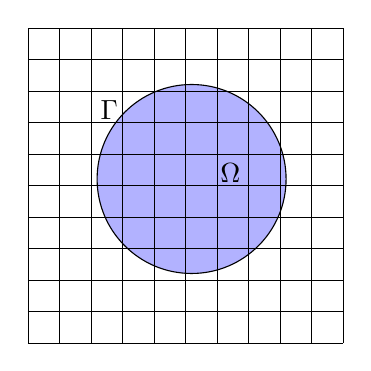
\begin{tikzpicture}[scale=0.80]
    \draw[fill=blue!30] (0.1, 0.1) circle (1.5cm);
    % Background mesh
    \foreach \i in {-2.5, -2, ..., 2.5} {
        \draw[line width=0.1pt, shift={(-2.5,\i)}] (0,0) -- (5,0);
        \draw[line width=0.1pt, shift={(\i,-2.5)}] (0,0) -- (0,5);
    }
    % Labels
    \node[below right] at (0.4,0.5) {$\Omega $};
    \node[below right] at (-1.5,1.5) {$\Gamma $};
\end{tikzpicture}
\caption{An illustration of a unfitted mesh.}
\label{fig:domain_unfitted_mesh}
\end{figure}

\begin{figure}
    \centering
    % First TikZ picture
    \begin{minipage}{0.45\textwidth}
        \centering
        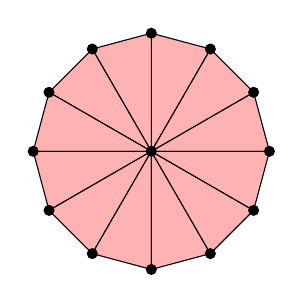
\begin{tikzpicture}
            % Circle
            % \draw (0, 0) circle (1.5cm);

            % Fitted mesh (crude triangular mesh)
            \foreach \i in {0, 30, ..., 330} {
                \draw[fill=red!30] (0, 0) -- (\i:1.5cm) -- (\i+30:1.5cm) -- cycle;
            }

            % Mesh nodes
            \foreach \i in {0, 30, ..., 330} {
                \fill[black] (\i:1.5cm) circle (2pt);
            }
            \fill[black] (0, 0) circle (2pt);
        \end{tikzpicture}
    \end{minipage}
    \hfill
    % Second TikZ picture
    \begin{minipage}{0.45\textwidth}
        \centering
        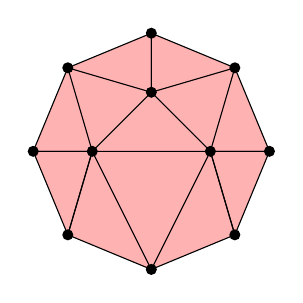
\begin{tikzpicture}
            % Boundary points
            \foreach \i in {0, 45, ..., 315} {
                \coordinate (boundary-\i) at (\i:1.5cm);
            }
            % Interior points
            \coordinate (interior-1) at (0.75, 0);
            \coordinate (interior-2) at (-0.75, 0);
            \coordinate (interior-3) at (0, 0.75);

            % Create a cycle connecting all the boundary points
            \fill[red!30] (boundary-0) -- (boundary-45) -- (boundary-90) -- (boundary-135) -- (boundary-180) -- (boundary-225) -- (boundary-270) -- (boundary-315) -- cycle;

            \foreach \i in {0, 45, ..., 315} {
                \fill[black] (\i:1.5cm) circle (2pt);
            }


            \fill[black] (interior-1) circle (2pt);
            \fill[black] (interior-2) circle (2pt);
            \fill[black] (interior-3) circle (2pt);


            % Triangulation (manually specified)
            \draw (boundary-0) -- (boundary-45) -- (interior-1) -- cycle;
            \draw (boundary-45) -- (boundary-90) -- (interior-3) -- cycle;
            \draw (boundary-90) -- (boundary-135) -- (interior-3) -- cycle;
            \draw (boundary-135) -- (boundary-180) -- (interior-2) -- cycle;
            \draw (boundary-180) -- (boundary-225) -- (interior-2) -- cycle;
            \draw (boundary-225) -- (boundary-270) -- (interior-2) -- cycle;
            \draw (boundary-270) -- (boundary-315) -- (interior-1) -- cycle;
            \draw (boundary-315) -- (boundary-0) -- (interior-1) -- cycle;

            % Triangulation between interior points
            \draw (interior-1) -- (interior-2) -- (interior-3) -- cycle;
        \end{tikzpicture}
    \end{minipage}
\caption{Examples of different triangulations for a fitted mesh for a circle.}
\label{fig:domain_fitted_mesh}
\end{figure}


% \begin{tikzpicture}
%     % Boundary points
%     \foreach \i in {0, 45, ..., 315} {
%         \coordinate (boundary-\i) at (\i:1.5cm);
%     }
%     % Interior points
%     \coordinate (interior-1) at (0.75, 0);
%     \coordinate (interior-2) at (-0.75, 0);
%     \coordinate (interior-3) at (0, 0.75);

%     % Create a cycle connecting all the boundary points
%     \fill[red!30] (boundary-0) -- (boundary-45) -- (boundary-90) -- (boundary-135) -- (boundary-180) -- (boundary-225) -- (boundary-270) -- (boundary-315) -- cycle;

%     \foreach \i in {0, 45, ..., 315} {
%         \fill[black] (\i:1.5cm) circle (2pt);
%     }

%     \fill[black] (interior-1) circle (2pt);
%     \fill[black] (interior-2) circle (2pt);
%     \fill[black] (interior-3) circle (2pt);

%     % Triangulation (manually specified)
%     \draw (boundary-0) -- (boundary-45) -- (interior-1) -- cycle;
%     \draw (boundary-45) -- (boundary-90) -- (interior-3) -- cycle;
%     \draw (boundary-90) -- (boundary-135) -- (interior-3) -- cycle;
%     \draw (boundary-135) -- (boundary-180) -- (interior-2) -- cycle;
%     \draw (boundary-180) -- (boundary-225) -- (interior-2) -- cycle;
%     \draw (boundary-225) -- (boundary-270) -- (interior-2) -- cycle;
%     \draw (boundary-270) -- (boundary-315) -- (interior-1) -- cycle;
%     \draw (boundary-315) -- (boundary-0) -- (interior-1) -- cycle;

%     % Triangulation between interior points
%     \draw (interior-1) -- (interior-2) -- (interior-3) -- cycle;

%     % Draw a square around the circle
%     \draw[blue] (-2.0cm, -2.0cm) rectangle (3.5cm, 2.0cm);

%     % Define rectangle node coordinates
%     \foreach \x [evaluate=\x as \xx using int(10*\x)] in {-2.0, -1.0, ..., 3.5} {
%       \foreach \y [evaluate=\y as \yy using int(10*\y)] in {-2.0, 2.0} {
%         \coordinate (rect-\xx-\yy) at (\x, \y);
%         \fill[black] (\x, \y) circle (2pt);
%       }
%     }
%     \foreach \y [evaluate=\y as \yy using int(10*\y)] in {-1.0, 0, 1.0} {
%       \foreach \x [evaluate=\x as \xx using int(10*\x)] in {-2.0, 2.3, 3.5} {
%         \coordinate (rect-\xx-\yy) at (\x, \y);
%         \fill[black] (\x, \y) circle (2pt);
%       }
%     }

%     % Draw triangulation using \rect-\x-\y notation for x = 2.3 and x = 3.5
%     % \draw (rect-23-20) -- (rect-35-20) -- (rect-23-0) -- cycle;
%     % \draw (rect-23-10) -- (rect-35-10) -- (rect-23-0) -- cycle;
%     % \draw (rect-23-0) -- (rect-35-0) -- (rect-23-10) -- cycle;
%     % \draw (rect-23-10) -- (rect-35-10) -- (rect-23-20) -- cycle;
%     % \draw (rect-23-20) -- (rect-35-20) -- (rect-35-10) -- cycle;

% \end{tikzpicture}
% \todo[inline]{ Fix triangulation. }

A crucial advantage of CutFEM is its ability to handle unfitted meshes, as illustrated in Figure 1, where the mesh does not conform to the domain boundary $\Gamma$. The biharmonic equation, which is a fourth-order PDE, arises in numerous applications, such as thin plate bending, and is relevant to the Cahn-Hilliard problem. The Cahn-Hilliard equation describes phase separation in binary alloys and is characterized by a fourth-order term, making it a suitable candidate for the application of CutFEM.

In contrast to the unfitted mesh in Figure \ref{fig:domain_unfitted_mesh}, Figure \ref{fig:domain_fitted_mesh} shows examples of fitted meshes, where the mesh conforms to the domain boundary. However, generating such meshes for complex geometries can be cumbersome and time-consuming. CutFEM offers a more flexible approach, enabling us to work with standard meshes and focus on the PDEs' discretization and the imposition of boundary conditions.

Mixed formulation of the biharmonic problem has been discussed here \cite{cai2023nitsche,burman2020cut}.


\subsection{Weak formulation}%
\label{sub:weak_formulation}

    \begin{figure}[htpb!]
        \centering
        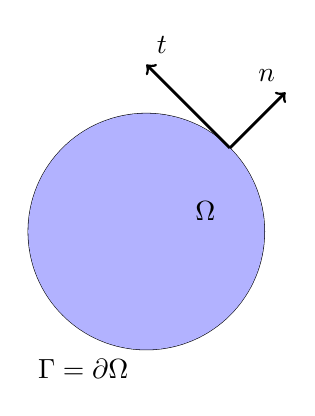
\begin{tikzpicture}
            % Circle
            \draw (0.0,0.0) circle (1.5cm);
            \fill[blue!30] (0.0,0.0) circle (1.5cm);

            \draw[->, line width=1.0pt] ({1.5*cos(45)}, { 1.5*sin(45) }) -- ({ 2.5*cos(45)  }, { 2.5*sin(45)  }) node[ above left] {$n $};
            \draw[->, line width=1.0pt] ({1.5*cos(45)}, { 1.5*sin(45) }) -- ({ 1.5*cos(45) - 1.5*sin(45) }, { 1.5*sin(45) + 1.5*cos(45) }) node[ above right] {$t $};

            % Labels
            \node[below right] at (0.5,0.5) {$\Omega$};
            \node[below right] at (-1.5,-1.5) {$\Gamma  = \partial \Omega$};
        \end{tikzpicture}
        \caption{ Illustration of an domain $\Omega $, the boundary $\Gamma $. The normal vector $n$  and the corresponding tangent vector.   }
        \label{fig:domain_construction}
    \end{figure}


    Let $\Omega \subseteq    \mathbb{R} ^d$ be a physical mesh, $\Gamma  $ be a $C^2$ boundary  illustrated at Figure \ref{fig:domain_construction}. Assume we have the function $\alpha: \Omega \to \mathbb{R} $. We define the strong biharmonic problem to be on the form

\begin{equation}
    \label{eq:Bi_strong}
\begin{split}
    \Delta^2  u  + \alpha  u  & = f( x)  \quad \text{in } \Omega,   \\
    \partial _{n} u & = g_{1}(x)   \quad \text{on } \Gamma ,  \\
    \partial _{n} \Delta  u & = g_2(x)  \quad \text{on } \Gamma  .  \\
\end{split}
\end{equation}

The goal is to write the problem on a weak form.
Let $u \in H^{4}( \Omega ) $ be a solution of the strong problem and $v \in H^{2}( \Omega ) $ be a test function. We argue that this holds,
    \[
        \begin{split}
(\Delta ^2u,v )_{\Omega } & = ( \partial _{n} \Delta u, v)_{\Gamma } - ( \nabla ( \Delta u) , \nabla v) _{\Gamma } \\
&= ( D^2u, D^2v)_{\Omega } + ( \partial _{n} \Delta u ,v)_{\Gamma } - ( \partial _{nn} u, \partial _{n}v)_{\Gamma } - ( \partial _{tn} u, \partial _{t} v)_{\Gamma }.        \\
        \end{split}
    \]
    Define the space $V_{g} = \left\{ u \in H^{2}( \Omega ) :  \partial _{n}u  \mid _{\Gamma } = g_1(x )  \right \} $ and $V = H^2( \Omega ) $.
    % By applying the boundary conditions can we see that $( \partial _{n} \Delta u, v)_\Gamma   = ( g,v)_{\Gamma }$ which occurs naturally. However, the Neumann boundary condition can be imposed by assuming $u \in V_{0}$ and
    %  as a consequence is the following terms $ ( \partial _{nn} u, \partial _{n}v)_{\Gamma }
    % = 0$   and $( \partial _{tn} u, \partial _{t}v)_{\Gamma } = 0$. This follows from the fact that that the Neumann boundary condition is homogeneous s.t. $\partial _{n} v = 0$ and $\partial _{t} (\partial _{n}u) = 0 $.
    % \todo[inline]{ But what if the Neumann conditions is not homogeneous? And why is it necessary to include it in the function space when it comes in "naturally"?  }
    Let $u,v \in V$ then is it natural to define an general bilinear form  \[
    a( u,v) = ( \alpha u,v)_{\Omega } +  ( D^2u, D^2v)_{\Omega }   .
    \]
    where $\alpha >0$ and a corresponding linear form $l: V \to \mathbb{R} $,
    \[
    l( v) = ( f ,v)_{\Omega  } -  ( g_{2},v)_{\Gamma } .
    \]
    We define the weak problem is to find a $u \in  V_{g}$ s.t. \[
    a( u,v) = l(v) \quad  \forall v \in V_{}
    \]







\subsection{Initial discrete formulation}%
\label{sub:initial_discrete_formulation}

We want to make a CutFEM version of the CIP problem. Let $\widetilde{\mathcal{T}_{h} } $ be a shape-regular and quasi-uniform background mesh. Let us denote the active set $\mathcal{T} _{h} \subseteq \widetilde{\mathcal{T}_{h}}$ which intersects the interior of the active domain $\Omega $, that is  \[
\mathcal{T} _{h} = \left\{ T \in \widetilde{\mathcal{T} }_{h}  \mid  T \cap (\Omega \setminus \Gamma ) \neq \emptyset    \right\} .
\]
With a corresponding set of interior facets, \[
    \mathcal{F} _{h} = \left\{ F = T^{+} \cap T^{-}  \mid  T^{+}, T^{-} \in \mathcal{T} _{h} \right\},
\]
and a set of cut elements \[
\mathcal{T} _{\Gamma } = \left\{ T \in \mathcal{T} _{h}   \mid  T \cap \Gamma \neq \emptyset  \right\}.
\]
For convenience, will we define also the interior of the active set as $\mathcal{T} _{int}$.
\[
\mathcal{T} _{int} = \left\{ T \in \mathcal{T} _{h}   \mid  T \cap  Int(\Omega ) \neq \emptyset  \right\}.
\]
Hence, we have that the active set is the union of the interior and cut elements, $\mathcal{T} _{h} = \mathcal{T} _{int} \cap \mathcal{T} _{\Gamma }$. For an illustration, see figure.


\begin{figure}\centering
\subfloat[]{\label{a}
        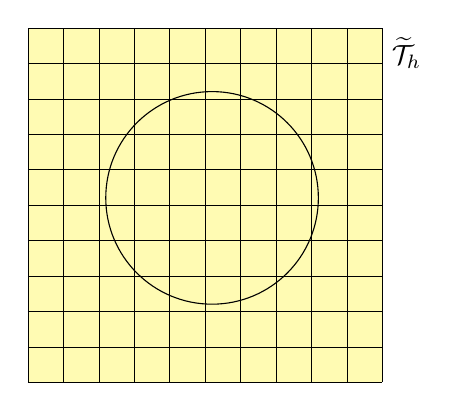
\begin{tikzpicture}[scale=0.9]

            \fill[yellow!30] (-2.5,2.5) -- (2.5,2.5) -- (2.5,-2.5) -- (-2.5,-2.5) -- cycle;

            \draw (0.1, 0.1) circle (1.5cm);
            % Background mesh
            \foreach \i in {-2.5, -2, ..., 2.5} {
                \draw[line width=0.1pt, shift={(-2.5,\i)}] (0,0) -- (5,0);
                \draw[line width=0.1pt, shift={(\i,-2.5)}] (0,0) -- (0,5);
            }


            % Labels
            \node[below right] at (2.5,2.5) {$\widetilde{\mathcal{T}}_{h}$};
        \end{tikzpicture}

}\hfill
\subfloat[]{\label{b}
        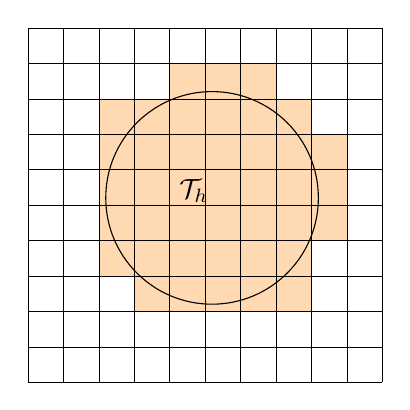
\begin{tikzpicture}[scale=0.9]

            % POTENTIAL ACTIVE MESH
            \fill[orange!30] (2,2) -- (2,-1.5) --(-1.5,-1.5) -- (-1.5,2) -- cycle;

            % ELEMENTS WITH NO INTERSECTION
            % lower left
            \fill[white] (-1.5,-1.5) rectangle (-1.0,-1.0);
            \fill[white] (-1.5,2.0) rectangle (-1.0,1.5);
            \fill[white] (-1.0,2.0) rectangle (-0.5,1.5);
            \fill[white] (2,2) rectangle (1.5,1.5);
            \fill[white] (1.5,2) rectangle (1.0,1.5);
            \fill[white] (2,1.5) rectangle (1.5,1.0);
            \fill[white] (1.5,-1) rectangle (2,-1.5);
            \fill[white] (1.5,-0.5) rectangle (2,-1.0);

            % CUT ELEMENTS
            \fill[orange!30] (-0.5,2.0) rectangle (1.0,1.5);
            \fill[orange!30] (-1.5,1.5) rectangle (0.0,1.0);
            \fill[orange!30] (0.5,1.5) rectangle (1.5,1.0);
            \fill[orange!30] (-1.5,1.0) rectangle (-1.0,-1.0);
            \fill[orange!30] (-1.0,-0.5) rectangle (-0.5,-1.5);
            \fill[orange!30] (-0.5,-1.5) rectangle (1.5,-1.0);
            \fill[orange!30] (1.5,-1) rectangle (1.0,-0.0);
            \fill[orange!30] (1.5,-0.5) rectangle (2.0,1.0);
            \fill[orange!30] (1.0,0.5) rectangle (1.5,1.0);

            \draw (0.1, 0.1) circle (1.5cm);
            % Background mesh
            \foreach \i in {-2.5, -2, ..., 2.5} {
                \draw[line width=0.1pt, shift={(-2.5,\i)}] (0,0) -- (5,0);
                \draw[line width=0.1pt, shift={(\i,-2.5)}] (0,0) -- (0,5);
            }


            % Labels
            % \node[below right] at (2.5,2.5) {$\widetilde{\mathcal{T}}_{h}$};
            % \node[below right] at (0.4,0.5) {$\mathcal{T}_{int}$};
            \node[below right] at (-0.5,0.5) {$\mathcal{T}_{h }$};
        \end{tikzpicture}


}\par

\subfloat[]{\label{c}
        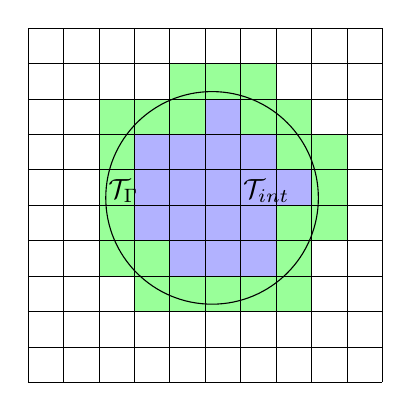
\begin{tikzpicture}[scale=0.9]

            % POTENTIAL ACTIVE MESH
            \fill[blue!30] (2,2) -- (2,-1.5) --(-1.5,-1.5) -- (-1.5,2) -- cycle;

            % ELEMENTS WITH NO INTERSECTION
            % lower left
            \fill[white] (-1.5,-1.5) rectangle (-1.0,-1.0);
            \fill[white] (-1.5,2.0) rectangle (-1.0,1.5);
            \fill[white] (-1.0,2.0) rectangle (-0.5,1.5);
            \fill[white] (2,2) rectangle (1.5,1.5);
            \fill[white] (1.5,2) rectangle (1.0,1.5);
            \fill[white] (2,1.5) rectangle (1.5,1.0);
            \fill[white] (1.5,-1) rectangle (2,-1.5);
            \fill[white] (1.5,-0.5) rectangle (2,-1.0);

            % CUT ELEMENTS
            \fill[green!40] (-0.5,2.0) rectangle (1.0,1.5);
            \fill[green!40] (-1.5,1.5) rectangle (0.0,1.0);
            \fill[green!40] (0.5,1.5) rectangle (1.5,1.0);
            \fill[green!40] (-1.5,1.0) rectangle (-1.0,-1.0);
            \fill[green!40] (-1.0,-0.5) rectangle (-0.5,-1.5);
            \fill[green!40] (-0.5,-1.5) rectangle (1.5,-1.0);
            \fill[green!40] (1.5,-1) rectangle (1.0,-0.0);
            \fill[green!40] (1.5,-0.5) rectangle (2.0,1.0);
            \fill[green!40] (1.0,0.5) rectangle (1.5,1.0);

            \draw (0.1, 0.1) circle (1.5cm);
            % Background mesh
            \foreach \i in {-2.5, -2, ..., 2.5} {
                \draw[line width=0.1pt, shift={(-2.5,\i)}] (0,0) -- (5,0);
                \draw[line width=0.1pt, shift={(\i,-2.5)}] (0,0) -- (0,5);
            }


            % Labels
            \node[below right] at (0.4,0.5) {$\mathcal{T}_{int}$};
            \node[below right] at (-1.5,0.5) {$\mathcal{T}_{\Gamma }$};
        \end{tikzpicture}
}

\caption{Illustration of the background mesh $\widetilde{T}_{h} $, the active set $\mathcal{T} _{h}$, the cut cells $\mathcal{T} _{\Gamma }$ and the interior of the active set $\mathcal{T} _{int}$ }
\label{fig:background_mesh}
\end{figure}





We denote the $C^{0}$ polynomial space of order $k$ as
\[
V_{h} = \left\{ v \in C^{0}\left( \Omega  \right): v_{T} = v | _{T} \in \mathcal{P} ^{k}\left( T \right), \forall T \in
\mathcal{T}_{h}    \right\}
\]




From the previous chapter can we write the CIP method. The bilinear form $a_{h}:  V_{h}\times  V_{h} \to \mathbb{R} $ is defined as

\begin{equation}
\label{eq:Bi_a_h}
\begin{split}
a_{h} \left( u, v \right)   =&   \left( \alpha  u, v \right) _{\mathcal{T} _{h} \cap \Omega }   +  \left( D^2 u, D^2v \right) _{\mathcal{T} _{h} \cap \Omega} \\
 & +
  \left( \mean{  \partial _{n n} u }, \jump{ \partial _{n }v} \right)_{\mathcal{F}_{h}^{} \cap \Omega}  +
 \left( \mean{ \partial _{n n} v }, \jump{ \partial _{n}u }      \right)_{\mathcal{F}_{h}^{} \cap \Omega} \\
 & + ( \partial _{nn} u, \partial _{n} v)_{\Gamma } + ( \partial _{nn} v, \partial _{n} u)_{\Gamma }
 \\
 & + \frac{\gamma }{h}  \left( \jump{ \partial _{n} u}, \jump{ \partial _{n} v_{}   }   \right)_{\mathcal{F}_{h}^{} \cap \Omega} +  \frac{\gamma }{h}  \left(  \partial _{n} u,  \partial _{n} v_{}      \right)_{\Gamma } \\
\end{split}
.
\end{equation}
Similarly the linear form is defined as
 \[
l_{h}( v) =  ( f,v)_{\mathcal{T} _{h} \cap \Omega } - (g_{2},v) - ( g_{1}, \partial _{nn}v) _{\Gamma } + \frac{\gamma }{h}  ( g_{1}, \partial _{n} v)   .
\]
To make sure the problem is stabilized will we add a ghost-penalty. That is, we define the discrete problem to find a $u_{h} \in V_{h}$ s.t. \[
A_{h}( u_{h} ,v ) := a_{h}( u_{h}, v)  + g_{h}( u_{h},v) = l_{h} ( v) \quad  \forall v \in  V_{h}.
\]
We define the underlying norms for $ v \in V_{h} $ as
    \begin{align}
        \label{eq:bi_ah_norm}
        \| v \|_{ a_{h} }^{ 2 } & =    \| |\alpha |^{\frac{1}{2}}  v \|_{ \mathcal{T} _{h} \cap \Omega  }^{ 2}  + \| D^2 v \|_{\mathcal{T} _{h} \cap \Omega   }^{ 2 } + \gamma \| h^{-\frac{1}{2}} \jump{ \partial _{n} v }   \|_{ \mathcal{F}_{h}^{}\cap \Omega    }^{ 2
        } + \gamma \| h^{-\frac{1}{2}}  \partial _{n} v    \|_{ \Gamma   }^{ 2 },    \\
        \label{eq:bi_gh_norm}
\abs{ v } _{g_{h}}^{2} & = g( v,v) \\
        \label{eq:bi_Ah_norm}
\| v \|_{A_{h}  }^{  2}  & = \| v \|_{ a_{h} }^{ 2 } + \abs{ v } _{g_{h}}^{2} \\
    \end{align}
and for $v \in V + V_{h}$ we get, \[
    \begin{split}
\| v \|_{ a_{h}, * }^{  2} & =\| v \|_{ a_{h} }^{ 2 } +  \| h^{\frac{1}{2}} \mean{ \partial _{nn} v }   \|_{\mathcal{F} _{h}^{} \cap \Omega   }^{  2} +  \| h^{\frac{1}{2}} \partial _{nn} v    \|_{ \Gamma }^{  2}  \\
\| v \|_{A_{h},*  }^{  2}  & = \| v \|_{ a_{h},* }^{ 2 } + \abs{ v } _{g_{h}}^{2}
    \end{split}
\]
\begin{remark}
Note that it holds that $\mathcal{T} _{h} \cap  \Omega   = \Omega  $ and $\mathcal{T} _{h} \cap  \Gamma  = \Gamma $. Depending on context, we choose the best suitable notation.
\end{remark}

\subsection{Stability estimate}%
\label{sub:stability_estimate}

Similarly for the Poisson problem will we have the following assumptions for the computational mesh;

\begin{enumerate}[label=\textbf{S.\arabic*}]
    \item\label{as:s1} Boundary $\Gamma $ is of $C^2$
    \item\label{as:s2} The mesh $\mathcal{T} _{h}$ is quasi-uniform.
    \item \label{as:s3}For a $T \in \mathcal{T} _{\Gamma }$ there exists a path $P$ of $diam(P) \lesssim h$ which contains $T$ and an element $T'$ with a so-called fat intersection $
    \abs{ T' \cap \Omega  } _{d} \ge \abs{ T' } _{d}$.
\end{enumerate}

From basic theory we have the following inverse estimate for $ v \in \mathcal{P}^{k}( T)$ s.t. \[
     \| \partial _{nn}  v \|_{F   }^{ }  \lesssim  \| h_{T}^{-\frac{1}{2}} D ^2 v \|_{ T }^{  },
\]
where the hidden constant depend on dimension $d$, order $k$ and the shape regularity. Similarly for cut elements is it easy to see that this must hold,
\begin{equation*}
     \| \partial _{nn}  v \|_{F \cap \Omega    }^{  }  \lesssim\| \partial _{nn}  v \|_{F }^{  }  \lesssim   \| h_{T}^{-\frac{1}{2}} D ^2 v \|_{ T }^{  }.
\end{equation*}
A useful variant is the following inequality that is,
\begin{equation*}
\| \partial _{nn} v \|_{ \Gamma \cap T  }^{  } \lesssim h^{-\frac{1}{2}} \| D^2 v \|_{ T }^{  }.
\end{equation*}
Summation the inverse inequalities over $\mathcal{F}_{h} $ and $\mathcal{T}_{h} $ implies that
\begin{align}
\label{eq:bi_cut_inverse_1}
\| \partial _{nn} v \|_{ \mathcal{T} _{h} \cap \Gamma  }^{  } &\lesssim h^{-\frac{1}{2}} \| D^2 v \|_{ \mathcal{T}_h }^{  }, \\
\label{eq:bi_cut_inverse_2}
\| \partial _{nn}  v \|_{ \mathcal{F}_h \cap \Omega    }^{  }  &  \lesssim   h^{-\frac{1}{2}} \| D^2 v \|_{ \mathcal{T}_h  }^{  }.
\end{align}
In fact, combining the inequalities we get the identity,
\begin{equation}
\label{eq:bi_identity}
h\| \partial _{nn}  v \|_{ \mathcal{F}_h \cap \Omega    }^{2 } + h\| \partial _{nn} v \|_{ \mathcal{T} _{h} \cap \Gamma  }^{2  } \lesssim \| D^2 v \|_{ \mathcal{T} _{h}  }^{2  }.
\end{equation}

We may introduce our first assumption on the ghost penalty.
\begin{assumption}[EP1]
    \label{as:bi_EP1}
    The ghost penalty $g_{h}$ extends the $H^{1}$ norm s.t. \[
    \| D^2 v \|_{ \mathcal{T} _{h} }^{ 2 } \lesssim  \| D^2 v \|_{ \Omega  }^{ 2 } + \abs{ v } _{g_{h}}^{2}.
    \]
\end{assumption}


Combing the results we get the following convenient corollary.

\begin{corollary}
    \label{cor:bi_inverse_thm}
    Let $g_{h}$ satisfy Assumption \ref{as:bi_EP1} then
    \[
            h\| \partial _{nn}  v \|_{ \mathcal{F}_h^{} \cap \Omega    }^{2 } + h\| \partial _{nn} v \|_{ \mathcal{T} _{h} \cap \Gamma  }^{2  }   \lesssim  \| D^2 v \|_{ \Omega  }^{ 2 } + \abs{ v } _{g_{h}}^{2} \\
              \lesssim \| v \|_{ A_{h} }^{  2}
    \]
\end{corollary}
\begin{proof}
    The first inequality is a direct result of \eqref{eq:bi_identity} and Assumption \ref{as:bi_EP1}. The second inequality is simply a results of the definition \eqref{eq:bi_Ah_norm}.
\end{proof}

\begin{lemma}
    \label{lemma:bi_Ah_coercive}
    The discrete form $A_{h}$ is coercive, that is, \[
    \| v \|_{ A_{h} }^{ 2 }  \lesssim A_{h}( v,v) \forall v \in V_{h}
    \]
\end{lemma}

\begin{proof}
    Let $v \in V^{h}$.
    Observe that \[
    A_{h}( v,v) = a_{h}( v,v)  + \abs{ v }_{g_{h}}^{2}
    \]
    Thus, since the second term already is part of the $\| \cdot  \|_{ A_{h} }^{  } $ norm is a good start to focus on the $a_{h}$ term, that is,
    \[
    \begin{split}
       a_{h}( v,v) &=   \|\ |\alpha|^{\frac{1}{2}} \cdot v  \|_{   \Omega   }^{2} + \| D^2v \|_{   \Omega  }^{2  } + 2 ( \mean{ \partial _{nn} v }, \jump{ \partial _{n} v }    )_{\mathcal{F} ^{}_{h} \cap \Omega }  + 2 (  \partial _{nn} v ,
       \partial _{n} v  )_{\Gamma } \\
                   & \quad+ \frac{\gamma }{h}  \|  \jump{ \partial _{n} v }\|_{\mathcal{F} _{h}^{}  }^{ 2 } + \frac{\gamma }{h}  \| \partial _{n} v \|_{ \Gamma  }^{ 2 }
    \end{split}
    \]
    We will first focus on the symmetry terms. Using Cauchy-Schwarz we observe that \[
        \begin{split}
    ( \mean{ \partial _{nn} v }  , \jump{ \partial _{n} v }  )_{\mathcal{F}^{}_{h}\cap \Omega  } & \ge - \| h^{\frac{1}{2}}\mean{ \partial _{nn} v }   \|_{ \mathcal{F}^{}_{h}\cap \Omega   }^{  }  \|h^{-\frac{1}{2}} \jump{ \partial _{n} v }   \|_{
    \mathcal{F}^{}_{h}\cap \Omega   }^{  } \\
    (  \partial _{nn} v   ,  \partial _{n} v   )_{\Gamma   } & \ge - \| h^{\frac{1}{2}} \partial _{nn} v    \|_{ \Gamma    }^{  }  \|h^{-\frac{1}{2}}  \partial _{n} v    \|_{ \Gamma    }^{  }
        \end{split}
    \]
    Using inverse-inequalities \eqref{eq:bi_cut_inverse_1} and \eqref{eq:bi_cut_inverse_2} and the Corollary \ref{cor:bi_inverse_thm} can we easily observe that \[
        \begin{split}
     \| \mean{ \partial _{nn}v } \|_{ \mathcal{T}_{h} \cap \Omega    }^{  2} & \le C_{1} \| D^2 v \|_{ \mathcal{T}_{h}   }^{2  } \le  C  (\| D^2 v \|_{ \Omega  }^{ 2 }  + \abs{ v } _{ g_{h} }^{2  } )  \\
     \|  \partial _{nn}v  \|_{ \Gamma     }^{ 2 } & \le C_{2} \| D^2 v \|_{ \mathcal{T} _{h}  }^{2  } \le C  (\| D^2 v \|_{ \Omega  }^{ 2 }  + \abs{ v } _{ g_{h} }^{2  } )
        \end{split}
    \]
    Thus, by applying Youngs $\varepsilon $-inequality, $2ab \le  \varepsilon^{-1} a^{2} + \varepsilon b^{2} $, is it natural to see that,
    \[
        \begin{split}
- C_{1}^{\frac{1}{2}} \| D^2 v    \|_{ \mathcal{T} _{h}   }^{  }  \|h^{-\frac{1}{2}} \jump{ \partial _{n} v }   \|_{ \mathcal{F}^{}_{h}\cap \Omega   }^{  }
& \ge - \frac{1}{\varepsilon } C  (\| D^2 v \|_{ \Omega  }^{ 2 }  + \abs{ v } _{ g_{h} }^{2  } ) -  \varepsilon \|h^{-\frac{1}{2}} \jump{ \partial _{n} v }   \|_{ \mathcal{F}^{}_{h}\cap \Omega   }^{2  } \\
- C_{2}^{\frac{1}{2}}  \| D^2 v \|_{ \mathcal{T} _{h} }^{  } \| h^{-\frac{1}{2}}  \partial _{n} v    \|_{ \Gamma    }^{  }
& \ge - \frac{1}{\varepsilon } C  (\| D^2 v \|_{ \Omega  }^{ 2 }  + \abs{ v } _{ g_{h} }^{2  } ) -  \varepsilon \|h^{-\frac{1}{2}}  \partial _{n} v    \|_{ \Gamma    }^{2  } \\
        \end{split}
    \]
    Combining these ideas do we end up with the following inequality,
    \[
    \begin{split}
       a_{h}( v,v)  \ge& \     \|\ |\alpha|^{\frac{1}{2}} \  v  \|_{   \Omega   }^{2} +\| D^2v  \|_{   \Omega   }^{2} -  \frac{1}{\varepsilon } 4C  (\| D^2 v \|_{ \Omega  }^{ 2 }  + \abs{ v } _{ g_{h} }^{2  } )  \\
                       & + (\gamma - 2\varepsilon  )\left( \|h^{-\frac{1}{2}}  \jump{ \partial _{n} v }\|_{\mathcal{F} _{h}^{} \cap \Omega   }^{ 2 } + \| h^{-\frac{1}{2}} \partial _{n} v \|_{ \Gamma  }^{ 2} \right)        \\
    \end{split}
    \]
    This inequality is useful, since if we apply it on the $\| \cdot  \|_{ A_{h} }^{  } $ we have a extra ghost penalty term s.t.,

    \[
        \begin{split}
     A_{h}( v,v) & = a( v,v) + \abs{ v }_{g_{h}}^{2} \\
     &\ge  \   \| \ |\alpha|^{\frac{1}{2}} \  v  \|_{   \Omega   }^{2} + (1  - \frac{1}{\varepsilon } 4C)  (\| D^2 v \|_{ \Omega  }^{ 2 }  + \abs{ v } _{ g_{h} }^{2  } )  \\
                       & + (\gamma - 2\varepsilon  )\left( \|h^{-\frac{1}{2}}  \jump{ \partial _{n} v }\|_{\mathcal{F} _{h}^{}\cap \Omega   }^{ 2 } + \| h^{-\frac{1}{2}} \partial _{n} v \|_{ \Gamma  }^{ 2} \right)        .
        \end{split}
    \]
    Setting $\varepsilon = 8C$ and $C=\frac{\gamma }{32} $ we simplify the problem to \[
        \begin{split}
           A_{h}( v,v)  \ge& \   \| \ |\alpha|^{\frac{1}{2}} \    v  \|_{  \Omega   }^{2} + \frac{1}{2}  (\| D^2 v \|_{ \Omega  }^{ 2 }  + \abs{ v } _{ g_{h} }^{2  } )  \\
                       & + \frac{\gamma }{2}\left( \|h^{-\frac{1}{2}}  \jump{ \partial _{n} v }\|_{\mathcal{F} _{h}^{}\cap \Omega   }^{ 2 } + \| h^{-\frac{1}{2}} \partial _{n} v \|_{ \Gamma  }^{ 2} \right) \\
                        \gtrsim & \  \| v \|_{ A_{h} }^{2  }
        \end{split}
    \]
    Hence, proof is complete.
\end{proof}


\begin{lemma}
    \label{lemma:bi_Ah_bounded}
    The discrete form $A_{h}$ is bounded, that is,
    \begin{equation}
    \label{eq:bi_A_h_bounded}
     A_{h}( v,w) \lesssim \| v \|_{A_{h}  }^{  }\| v \|_{A_{h}  }^{  }  \forall w \in V_{h}
    \end{equation}
    Moreover, for $v \in V_{h} + V$  and $w \in V_{h}$ the discrete form $a_{h}$ satisfies
    \begin{equation}
        \label{eq:bi_a_h_bounded}
        a_{h} ( v,w) \lesssim \| v \|_{ a_{h},* }^{  } \| w \|_{ A_{h} }^{  }
    \end{equation}
\end{lemma}

\begin{proof}
    We will divide the proof in two steps.
    \begin{enumerate}[label=\arabic*)]
        \item The goal is to prove the inequality \eqref{eq:bi_A_h_bounded}. \[
                \abs{ A_{h}( v ,w ) } \lesssim   \abs{a_{h}( v, w) }   + \abs{g_{h}( v,w)  }          \]
                By assumption is the ghost penalty $g_{h}$ positive semi-definite, thus, it fulfills the Cauchy-Schwartz inequality \[
                \abs{ g_{h}(v,w ) } \lesssim \abs{ v } _{g_{h}}\abs{ w }_{g_{h}}
                \]
                Hence, by definition is $\abs{ g_{h}(v,w ) } \lesssim \| v \|_{ A_{h} }^{  } \| w \|_{ A_{h} }^{  } $. Now it remains to show that the bilinear term $ a_{h}$ is bounded.
                \begin{equation}
                    \begin{split}
                        \abs{ a_{h} \left( v, w \right) }   \le  &   \abs{\left( \alpha  v, w \right) _{\mathcal{T} _{h} \cap \Omega }  }    +  \abs{\left( D^2 v, D^2w \right) _{\mathcal{T} _{h} \cap \Omega}  }  \\
                                                     & + \abs{\left( \mean{  \partial _{n n} v }, \jump{ \partial _{n }w} \right)_{\mathcal{F}_{h}^{} \cap \Omega}  }   +
                                                     \abs{\left( \mean{ \partial _{nn } v }, \jump{ \partial _{n}w }      \right)_{\mathcal{F}_{h}^{} \cap \Omega}  } \\
                                                     & + \abs{\left(  \partial _{n n} v ,  \partial _{n }w \right)_{\Gamma }}     +
                                                     \abs{\left(  \partial _{n n} w ,  \partial _{n}v       \right)_{\Gamma }  }
                                                     \\
                                                     & + \frac{\gamma }{h} \abs{ \left( \jump{ \partial _{n} v}, \jump{ \partial _{n} w   }   \right)_{\mathcal{F}_{h}^{} \cap \Omega}  } + \frac{\gamma }{h} \abs{ \left(  \partial _{n} v,  \partial _{n} w
                                                     \right)_{\Gamma }  }
                    \end{split}
                \end{equation}
                The strategy is to bound each term individually using Cauchy-Schwartz. We can easily see that $\abs{\left( \alpha  v, w \right) _{\mathcal{T} _{h} \cap \Omega }  }   \lesssim \| v \|_{a_{h}  }^{  } \| w \|_{ a_{h} }^{  } $ and that
                $\abs{\left( D^2 v, D^2w \right) _{\mathcal{T} _{h} \cap \Omega}  } \lesssim \| v \|_{a_{h}  }^{  } \| w \|_{ a_{h} }^{  } $ using Cauchy Schwartz. For the symmetric terms we also apply the inverse inequality
                \eqref{eq:bi_cut_inverse_2}.
                \[
                    \begin{split}
                    \abs{\left( \mean{ \partial _{n n} v }, \jump{ \partial _{n}w }      \right)_{\mathcal{F}_{h}^{} \cap \Omega}  } & \lesssim  \|\mean{ \partial _{n n} v }  \|_{ \mathcal{F}_{h}^{} \cap \Omega}^{  }\|\jump{ \partial _{n} w }  \|_{
                    \mathcal{F}_{h}^{} \cap \Omega}^{  } \\
                    & \lesssim  \|h^{\frac{1}{2}} \partial _{n n} v  \|_{ \mathcal{F}_{h}^{} \cap \Omega}^{  }\| h^{-\frac{1}{2}} \jump{ \partial _{n} w }     \|_{\mathcal{F}_{h}^{} \cap \Omega}^{  } \\
                    & \lesssim  \| v \|_{A_{h}  }^{  } \|w    \|_{ a_{h}}^{  }
                    \end{split}
                \]
                Here we used the Corollary \ref{cor:bi_inverse_thm} s.t.  $\|h^{\frac{1}{2}} \partial _{n n}  v \|_{\mathcal{F}_{h}^{} \cap \Omega} \lesssim \| v \|_{ A_{h}  }^{  }  $.
              The boundedness interior penalty  inequality is showed in this manner, \[
             \frac{\gamma }{h} \abs{ \left( \jump{ \partial _{n} v}, \jump{ \partial _{n} w   }   \right)_{\mathcal{F}_{h}^{} \cap \Omega}  }  \lesssim  \|h^{-\frac{1}{2}} \jump{ \partial _{n} v}  \|_{ \mathcal{F}_{h}^{} \cap \Omega }^{  }
             \|h^{-\frac{1}{2}} \jump{ \partial _{n} w}  \|_{ \mathcal{F}_{h}^{} \cap \Omega }^{  }  \lesssim  \| v  \|_{ a_{h} }^{  }
             \| w  \|_{ a_{h} }^{  }.
             \]
              Now it remains to handle boundary terms. \[
                \abs{ ( \partial _{nn} v, \partial _{n} w)_{\Gamma } }  \lesssim \| h^{\frac{1}{2}}\partial _{nn} v \|_{\Gamma   }^{  } \| h^{-\frac{1}{2}} \partial _{n}w \|_{\Gamma   }^{  }  \lesssim \|  v \|_{A_{h}  }^{  } \| w \|_{ a_{h}   }^{  }
             \]
             Again, here we used the Corollary \ref{cor:bi_inverse_thm}.
             Finally, using the definition of the norm is it easily to see that,
             \[
\frac{\gamma }{h} \abs{ \left(  \partial _{n} v,  \partial _{n} w \right)_{\Gamma }  } \lesssim \gamma  \| h^{-\frac{1}{2}} \partial _{n} v \|_{  \Gamma }^{  } \| h^{-\frac{1}{2}} \partial _{n} w \|_{\Gamma   }^{  } \lesssim \| v \|_{ a_{h} }^{  }
\| w \|_{ a_{h} }^{  } .
             \]

             Obviously is $\| v \|_{a_{h}  }^{  } \lesssim \| v \|_{A_{h}  }^{  }$. Hence, we have showed that all terms in $a_{h}$ is bounded in the $\|\cdot   \|_{A_{h}  }^{  } $ norm.
         \item The goal is to prove \eqref{eq:bi_a_h_bounded} using many of the same ideas as in the first part. Let $v \in V_{h} +V $ and $v \in V_{h}$. Next step is to show that the bilinear term $ a_{h}$ is bounded.
                \begin{equation}
                    \begin{split}
                        \abs{ a_{h} \left( v, w \right) }   \le  &   \abs{\left( \alpha  v, w \right) _{\mathcal{T} _{h} \cap \Omega }  }    +  \abs{\left( D^2 v, D^2w \right) _{\mathcal{T} _{h} \cap \Omega}  }  \\
                                                     & + \abs{\left( \mean{  \partial _{n n} v }, \jump{ \partial _{n }w} \right)_{\mathcal{F}_{h}^{} \cap \Omega}  }   + \abs{\left( \mean{ \partial _{nn } w }, \jump{ \partial _{n}v }
                                                     \right)_{\mathcal{F}_{h}^{} \cap \Omega}  } \\
                                                     & + \abs{\left(  \partial _{n n} v ,  \partial _{n }w \right)_{\Gamma }}     +
                                                     \abs{\left(  \partial _{n n} w ,  \partial _{n}v       \right)_{\Gamma }  }
                                                     \\
                                                     & + \frac{\gamma }{h} \abs{ \left( \jump{ \partial _{n} v}, \jump{ \partial _{n} w   }   \right)_{\mathcal{F}_{h}^{} \cap \Omega}  } + \frac{\gamma }{h} \abs{ \left(  \partial _{n} v,  \partial _{n} w
                                                     \right)_{\Gamma }  }
                    \end{split}
                \end{equation}
                     We can easily observe from the first part that this must holds, \[
    \abs{\left( \alpha  v, w \right) _{\mathcal{T} _{h} \cap \Omega }  }    +  \abs{\left( D^2 v, D^2w \right) _{\mathcal{T} _{h} \cap \Omega}  } \lesssim \| v \|_{ a_{h},* }^{  } \| w \|_{A_{h}  }^{  }.
    \]
    And for the symmetric interior terms,
    \[
        \begin{split}
            \abs{\left( \mean{  \partial _{n n} v }, \jump{ \partial _{n }w} \right)_{\mathcal{F}_{h}^{} \cap \Omega}  } &\lesssim \| h^{\frac{1}{2}}\mean{ \partial _{nn}v }   \|_{ \mathcal{F}_{h}^{} \cap \Omega  }^{  } \| h^{-\frac{1}{2}}\jump{ \partial _{n }w}
    \|_{\mathcal{F}_{h}^{} \cap \Omega  }^{  } \lesssim \| v  \|_{ a_{h},*  }^{  }\|  w \|_{A_{h}  }^{  }, \\
            \abs{\left( \mean{  \partial _{n n} w }, \jump{ \partial _{n }v} \right)_{\mathcal{F}_{h}^{} \cap \Omega}  } &\lesssim \| h^{\frac{1}{2}}\mean{ \partial _{nn}w }   \|_{ \mathcal{F}_{h}^{} \cap \Omega  }^{  } \| h^{-\frac{1}{2}}\jump{ \partial _{n }v}
    \|_{\mathcal{F}_{h}^{} \cap \Omega  }^{  } \lesssim \| w  \|_{A_{h}  }^{  }\|  v \|_{ a_{h},*  }^{  }.
        \end{split}
    \]
    Remark that for $\| h^{\frac{1}{2}} \mean{ \partial _{nn} v }   \|_{\mathcal{F}^{} _{h} \cap \Omega   }^{  } $ is the norm incorporated in the definition of $\| \cdot  \|_{ a_{h},* }^{  } $, but for $\| h^{\frac{1}{2}} \mean{ \partial _{nn} w }   \|_{
    \mathcal{F}_{h}^{}\cap \Omega   }^{  } $ was the Corollary \ref{cor:bi_inverse_thm} applied. The jump terms $\|h^{-\frac{1}{2}} \jump{\partial _{n} v  }   \|_{\mathcal{F}^{}_{h}\cap \Omega    }^{  } $
is incorporated in the $\| \cdot  \|_{ a_{h} }^{  } $ norm, thus, this also holds, \[
\frac{\gamma }{h}\abs{  ( \jump{ \partial _{n} v }  , \jump{\partial _{n} w }  )_{\mathcal{F}^{} _{h} \cap \Omega } } \lesssim \| h^{-\frac{1}{2}} \jump{\partial _{n} v },      \|_{ \mathcal{F}^{} _{h}\cap \Omega   }^{  }     \|
h^{-\frac{1}{2}} \jump{\partial _{n} w } \|_{\mathcal{F}^{} _{h}\cap \Omega
}^{  } \lesssim \| v \|_{ a_{h},* }^{  } \| w \|_{ A_{h} }^{  }
\]
Finally, the boundary terms, \[
    \begin{split}
( \partial _{nn} v, \partial _{n} w)_\Gamma & \lesssim \| h^{\frac{1}{2}} \partial _{nn} v \|_{ \Gamma   }^{  }  \|h^{-\frac{1}{2}} \partial _{n} w \|_{ \Gamma   }^{  } \lesssim \| v \|_{ a_{h},* }^{  } \| w \|_{ A_{h} }^{  }   , \\
( \partial _{nn} w, \partial _{n} v)_\Gamma & \lesssim \| h^{\frac{1}{2}} \partial _{nn} w \|_{ \Gamma   }^{  }  \|h^{-\frac{1}{2}} \partial _{n} v \|_{ \Gamma   }^{  } \lesssim \| w \|_{ A_{h} }^{  } \| v \|_{ a_{h},* }^{  }   , \\
    \end{split}
\]
and \[
\frac{\gamma }{h} \abs{ (  \partial _{n} v, \partial _{n}w)_{\mathcal{F}^{} _{h} \cap \Omega }   }\lesssim \| h^{- \frac{1}{2}} \partial _{n} v \|_{ \Gamma   }^{  }  \| h^{-\frac{1}{2}} \partial _{n} w \|_{ \Gamma   }^{  } \lesssim \| v \|_{ a_{h},*
}^{  } \| w \|_{ A_{h}  }^{  },
\]
where we just applied the definition of the norms $\| \cdot  \|_{a_{h}  }^{  } $ and $\| \cdot  \|_{a_{h},*  }^{  } $. We have now shown that every term is bounded.

    \end{enumerate}
    Hence, the proof is complete.
\end{proof}

    % \todo[inline]{ Why is not $\| \mean{ \partial _{nn} v}   \|_{\mathcal{F}_h^{}  }^{  } \lesssim \|  \partial _{nn} v   \|_{ \mathcal{F}^{} }^{  }  $ interesting for $v \in V + V_h$, but is often used for $v \in V$?  Ex. the mean is conserved in the $\|
    % \cdot \|_{a_h,*}$ norm}



